\subsection{Internationalization}
\subsubsection{Overview}The bigger your web service is, the more attention you
should pay to make it more accessible to other users. One of the main barrier is language. Because of MVC model we split the application into logic, behavior and view, but there is sometimes a need for a next partition.

Creating multi-lingual service we should only focus on changing the content we want to display - the view should remain always the same. E\_lang provides a very convenient API to keep views the same and switch only the dictionary which application uses for each request.

E\_lang has been built upon a key-value mapping. Basic idea is to use only the keys in our application instead of language-specific elements and place all the translation in the separate files.

Keys for translation used within application are strings, which can be parsed in two ways:
\begin{description}
\item[string contains ":"] - string is split by {\bf :} character and the actual key is a tuple of string - tokens created by splitting the original string
\item[string doesn't contain ":"] - string is the key
\end{description}

Language files are read into memory during the start of the application, so after any change in those files there is a need to reload them. It could be done by calling
\begin{verbatim}
e_lang:reinstall().
\end{verbatim}

\subsubsection{Defining translations}
\paragraph{Preparing {\em project.conf}}First step of translating process is to put {\it language\_files} tuple in {\it project.conf} file. This two-element tuple should be in the following format:

%\begin{quotation}
\{language\_files, $\left[ {\bf LanguageFileSpec} | \ldots | \ldots \right]$ \}
%\end{quotation}

where {\bf LanguageFileSpec} is
%\begin{verbatim}
\{{\bf LangCode}, {\bf PathToTranslationFile}\}
%\end{verbatim}
{\bf LangCode} is an atom representing the language of the translation file.

\paragraph{Preparing translation files}Secondly, we should create all files we specified in {\it project.conf} and place there translations for all the keys we used in our application.

Translation file contains Erlang tuples in format:
%\begin{verbatim}
\{{\bf Key}, {\bf Translation}\}
%\end{verbatim}
where {\bf Key} is either a single string or a tuple of strings (look at {\it Overview} section).

\subsubsection{Translating} There are three ways of accessing translated strings:
\begin{itemize}
\item We can use $<$wpart:lang key=Key /$>$ inside the {\it html} file. During the process of tags expanding this tag will be replaced with the proper translation.
\item Call {\bf wpart\_lang:get\_translation/1} with key we want to translate.
\item Use tuple \{key, {\bf Key}\} in {\it description} option in {\it .hrl} record definition file.
\end{itemize}

\subsubsection{Control flow} All types of translating (using wpart, specifying description in {\it .hrl} files and explicitly calling {\it get\_translation} function) has the same control flow.

The target language is chosen in the following order:
\begin{enumerate}
\item from {\bf lang} key kept in {\bf session} in {\bf e\_dict}
\item from {\bf default\_language} option in {\it project.conf} file
\item if none of this options is set, e\_lang assumes we want to use English ({\it en} language code)
\end{enumerate}
Language codes used in application must be the same as those declared in {\it project.conf}.

Translation process behaves as follows:
\begin{enumerate}
\item if translation for given key is found, it is returned
\item otherwise, if key is a single string (not a tuple), the key is returned
\item in other cases "no translation found" string is returned
\end{enumerate}

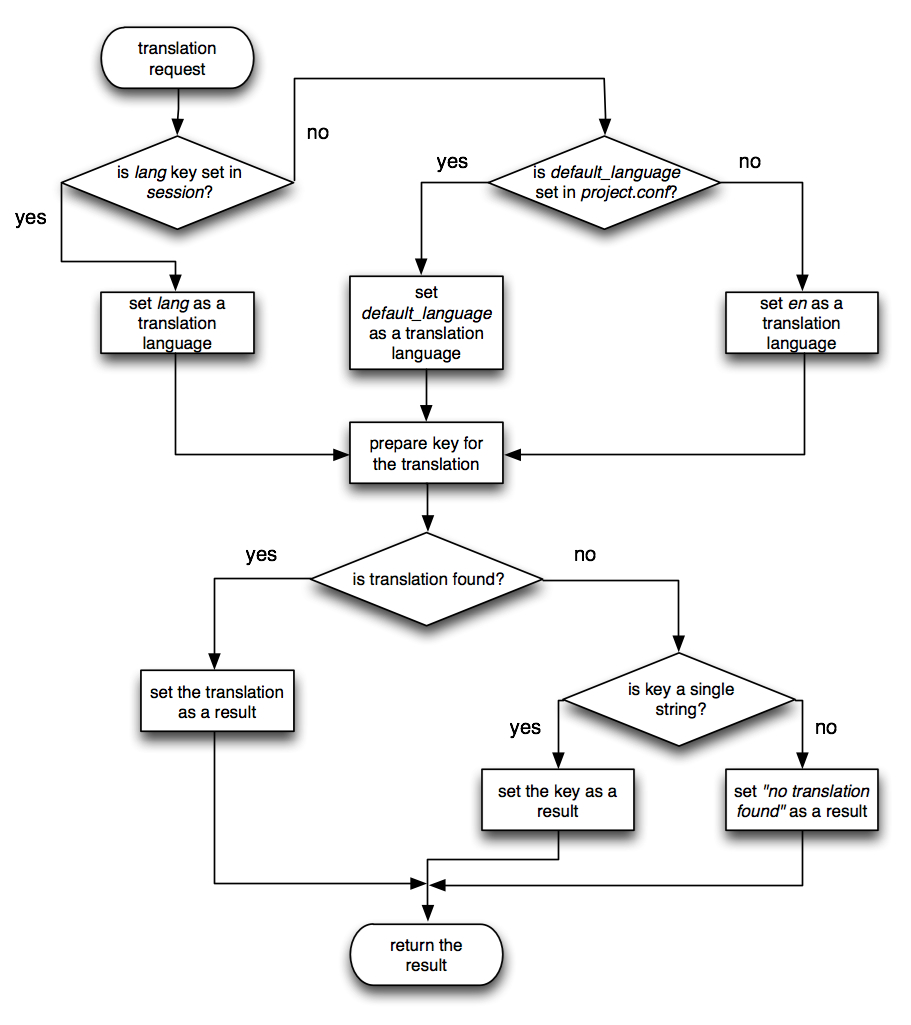
\includegraphics[width=\textwidth]{images/e_lang.jpg}   

\clearpage
\subsubsection{Example}
\paragraph{html embedding} 
\begin{Verbatim}[numbers=left]
...
<h1><wpart:lang key="contact:header"/></h1>
erlangweb@example.org<br/>
<wpart:lang key="back"/>
...
\end{Verbatim}
In this example two translations will be used: one with key {\it \{"contact", "header"\}} and one with {\it "back"}.

\paragraph{get\_translation call}
\begin{Verbatim}[numbers=left]
...
ErrorMsg = wpart_lang:get_translation("errors:no_such_login"),
...
\end{Verbatim}
{\bf ErrorMsg} variable will be bound to the translation corresponding to the {\it \{"errors", "no\_such\_login"\}} key.

\paragraph{description option in record definition file}
\begin{Verbatim}[numbers=left]
...
-record(login_types,
        {login = {string, [{description, {key, "login:login"}}]},
         password = {password, [{description, {key, "login:password"}}]}}).
...
\end{Verbatim}
Descriptions for {\it \#login\_types.login} and {\it \#login\_types.password} will be found under the keys {\it \{"login", "login"\}} and {\it \{"login", "password"\}} respectively.

\paragraph{language configuration file: "en.conf"}
\begin{Verbatim}[numbers=left]
{{"contact", "header"}, "My contact details"}.
{"back", "Go Back"}.
{{"errors", "no_such_login"}, "There is no such user in the system"}.
{{"login", "login"}, "Login"}.
{{"login", "password"}, "Password"}.
\end{Verbatim}

This file includes all the translations for the examples quoted above.
